\chapter{Perancangan Model SysML}
Setiap gambar adalah hasil render source Mermaid atau PlantUML. Bentuk renderer dipetakan secara eksplisit ke elemen SysML; gambar bukan sumber semantik yang berdiri sendiri. Model menggunakan ID konsisten dan stereotype/annotation yang dijelaskan dalam traceability. Gambar~\ref{fig:requirements} sampai Gambar~\ref{fig:ibd} menyajikan tujuh view.
\section{Requirement view}
Requirement view menampilkan empat requirement inti dengan dependency satisfy dan satu verify. Seluruh 24 requirement tetap terdaftar dan terhubung pada katalog serta matrix; ini partial view, bukan penghilangan requirement.
\begin{figure}[htbp]\centering
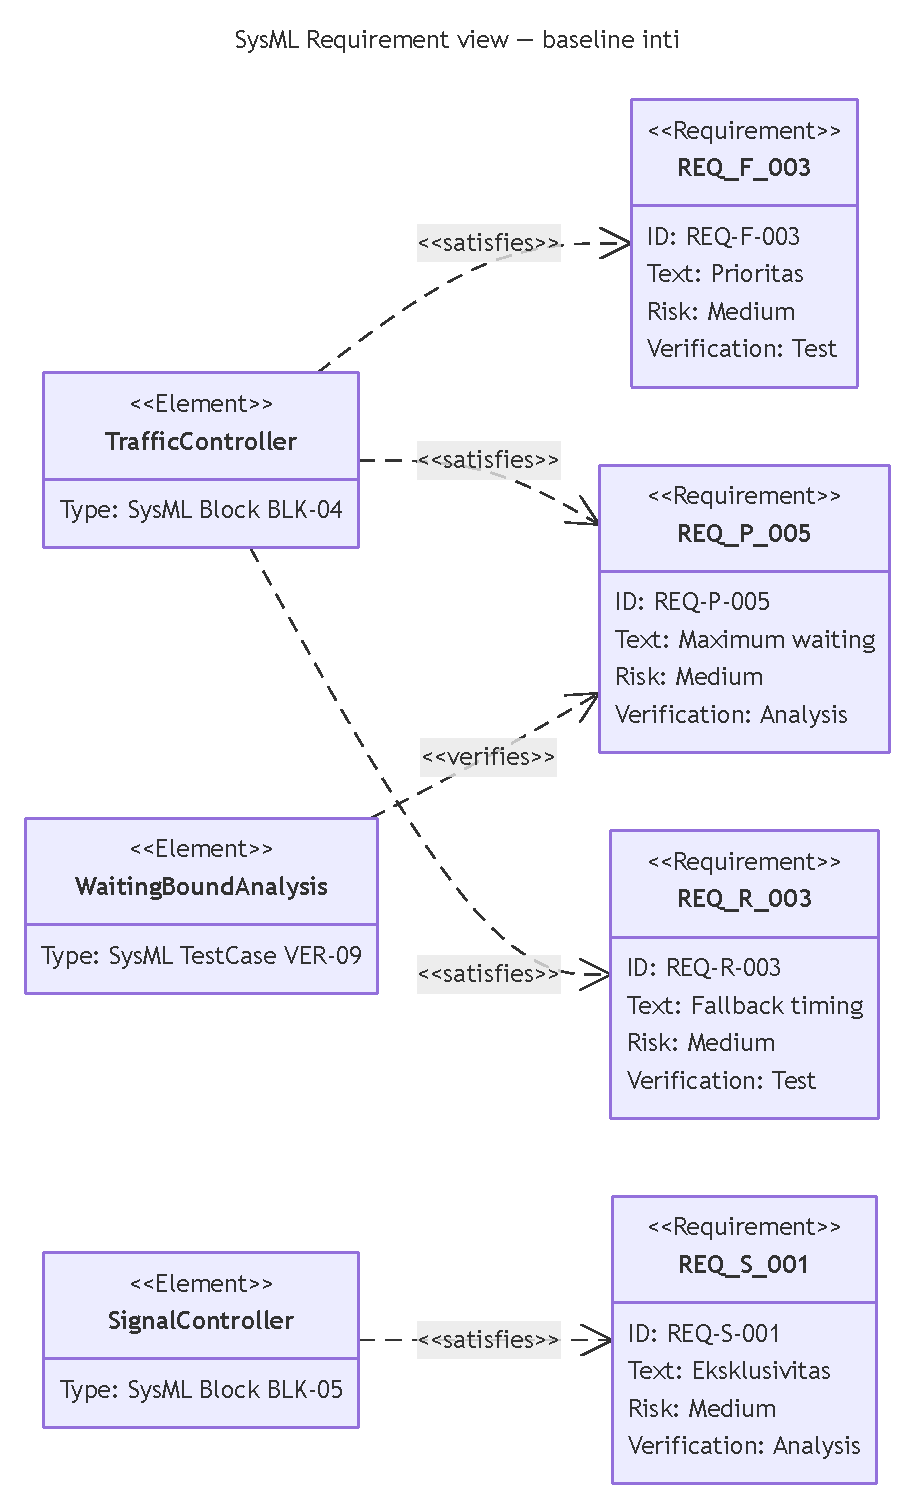
\includegraphics[width=\linewidth,height=.60\textheight,keepaspectratio]{requirements.pdf}
\caption{Requirement view dari model baseline}\label{fig:requirements}
\sumber{Pemodelan proyek berdasarkan asumsi desain ASM-001--010 (2026)}
\end{figure}
\clearpage
\clearpage
\begin{landscape}
\section{Use case view}
UC-02 mencakup MaintainSafeSignals, sedangkan HandleDataFailure memperluas pelayanan pada kondisi dataFault. TrafficDataSource tetap di luar boundary; komponen internal tidak dijadikan actor.
\begin{figure}[htbp]\centering
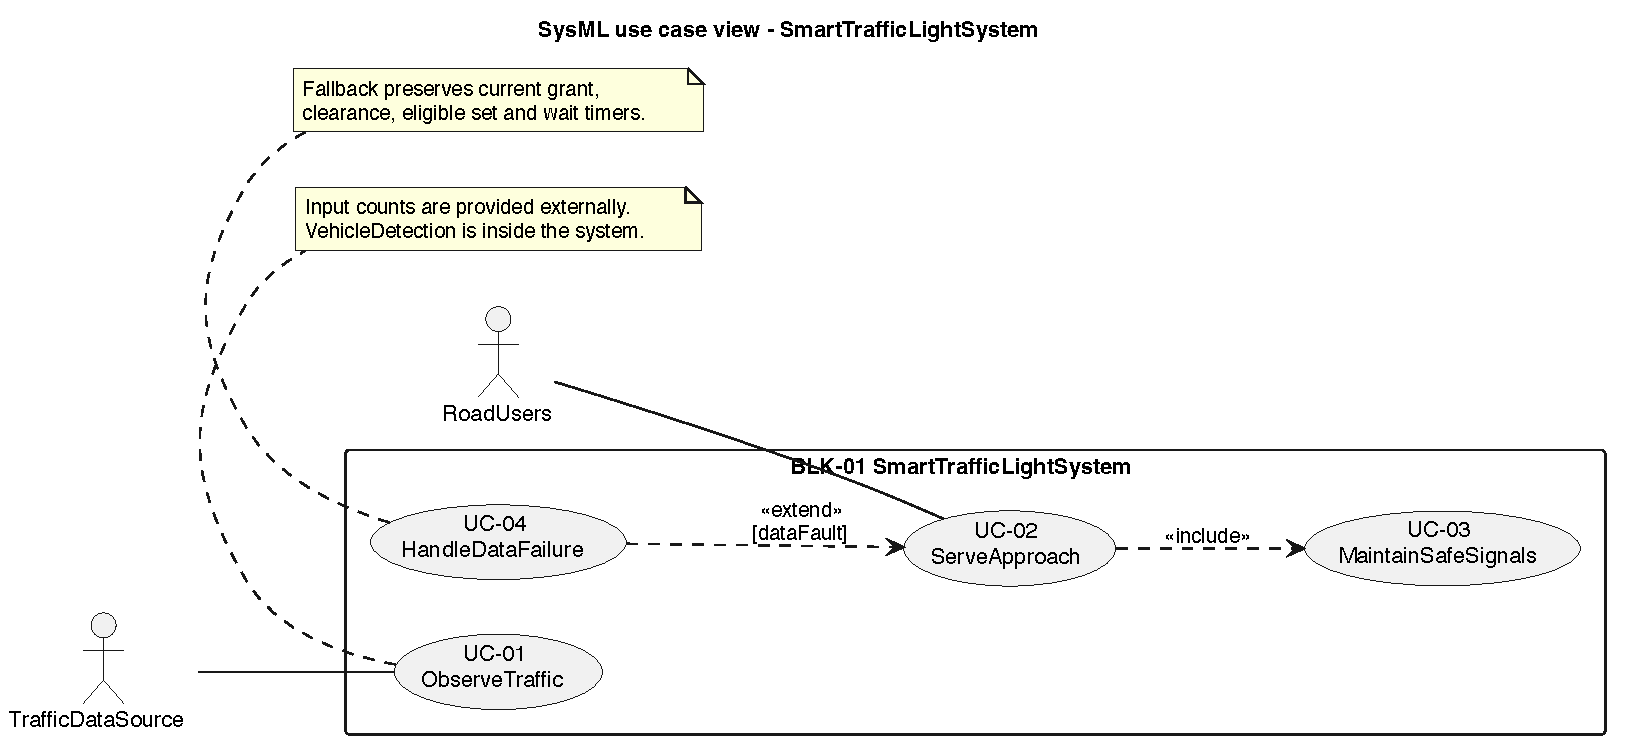
\includegraphics[width=\linewidth,height=.66\textwidth,keepaspectratio]{use-case.pdf}
\caption{Use case view dari model baseline}\label{fig:use-case}
\sumber{Pemodelan proyek berdasarkan asumsi desain ASM-001--010 (2026)}
\end{figure}
\clearpage
\end{landscape}
\clearpage
\section{Activity view}
Alokasi action ke block tercantum pada dictionary model. Loop menerima event sample atau phase timer; transisi clearance hanya berjalan bila event STM-01 mengaktifkannya, bukan delay blocking setiap sampel.
\begin{figure}[htbp]\centering
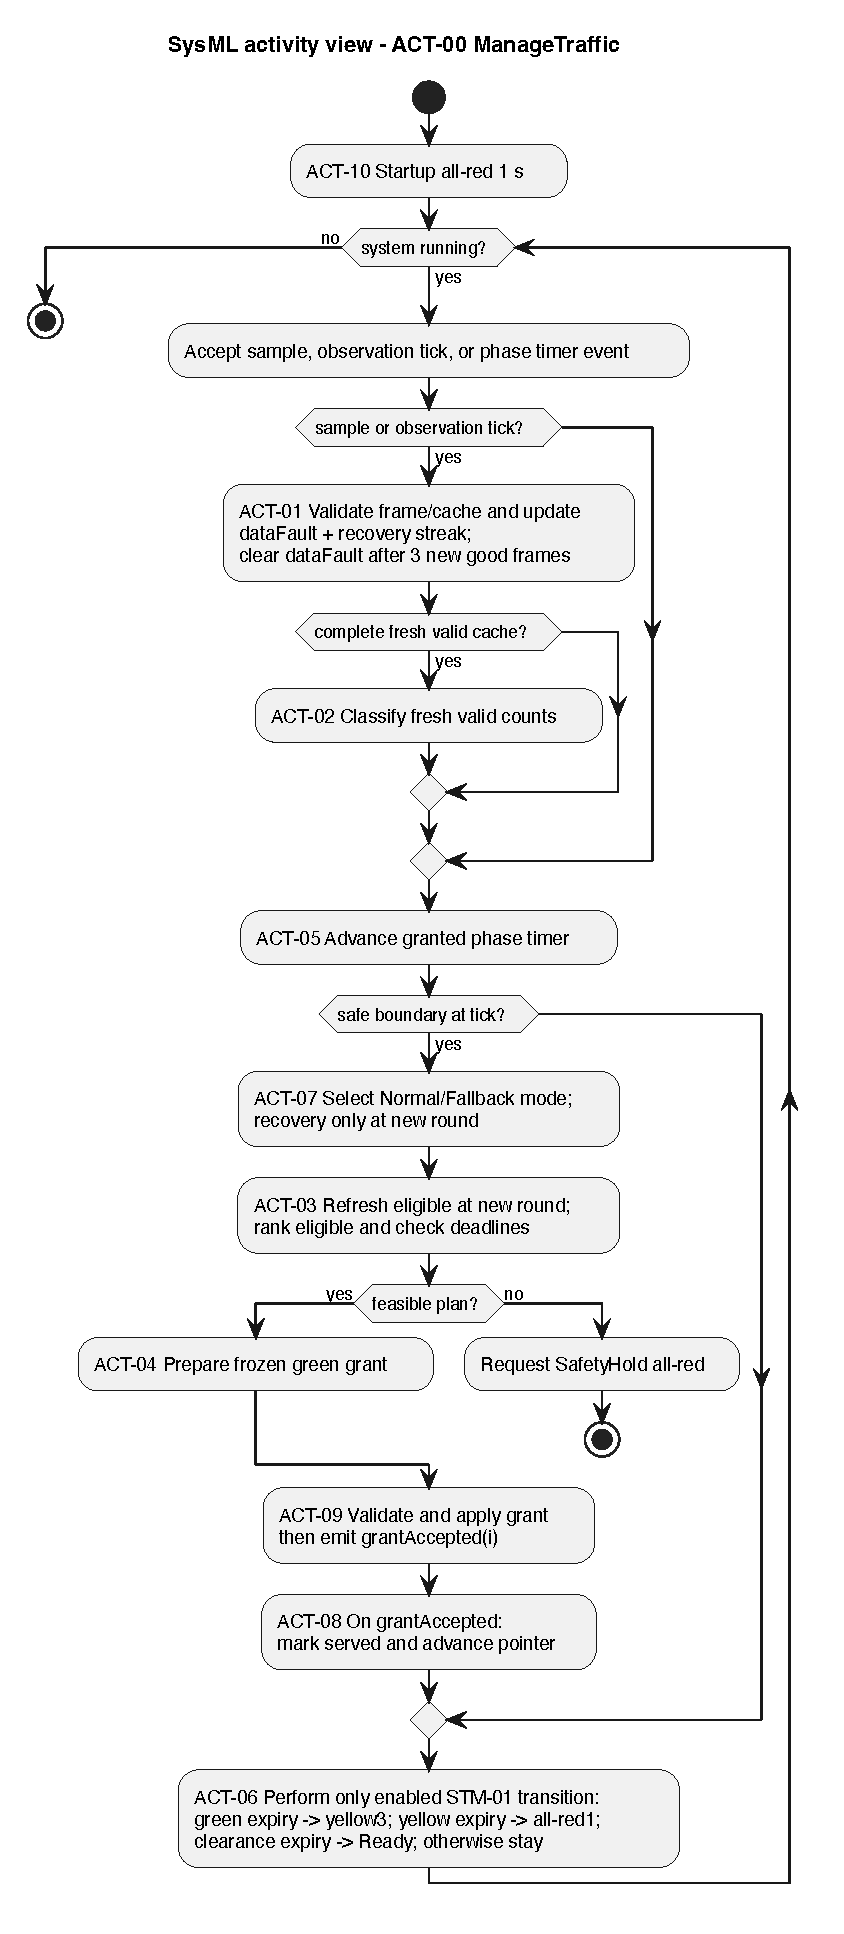
\includegraphics[width=\linewidth,height=.76\textheight,keepaspectratio]{activity.pdf}
\caption{Activity view dari model baseline}\label{fig:activity}
\sumber{Pemodelan proyek berdasarkan asumsi desain ASM-001--010 (2026)}
\end{figure}
\clearpage
\clearpage
\begin{landscape}
\section{Sequence view}
Lifeline mereferensikan part yang sama dengan IBD. DataFault dilatch selama green, tetapi grant tetap sampai timer berakhir; mode berikutnya diputuskan pada boundary aman.
\begin{figure}[htbp]\centering
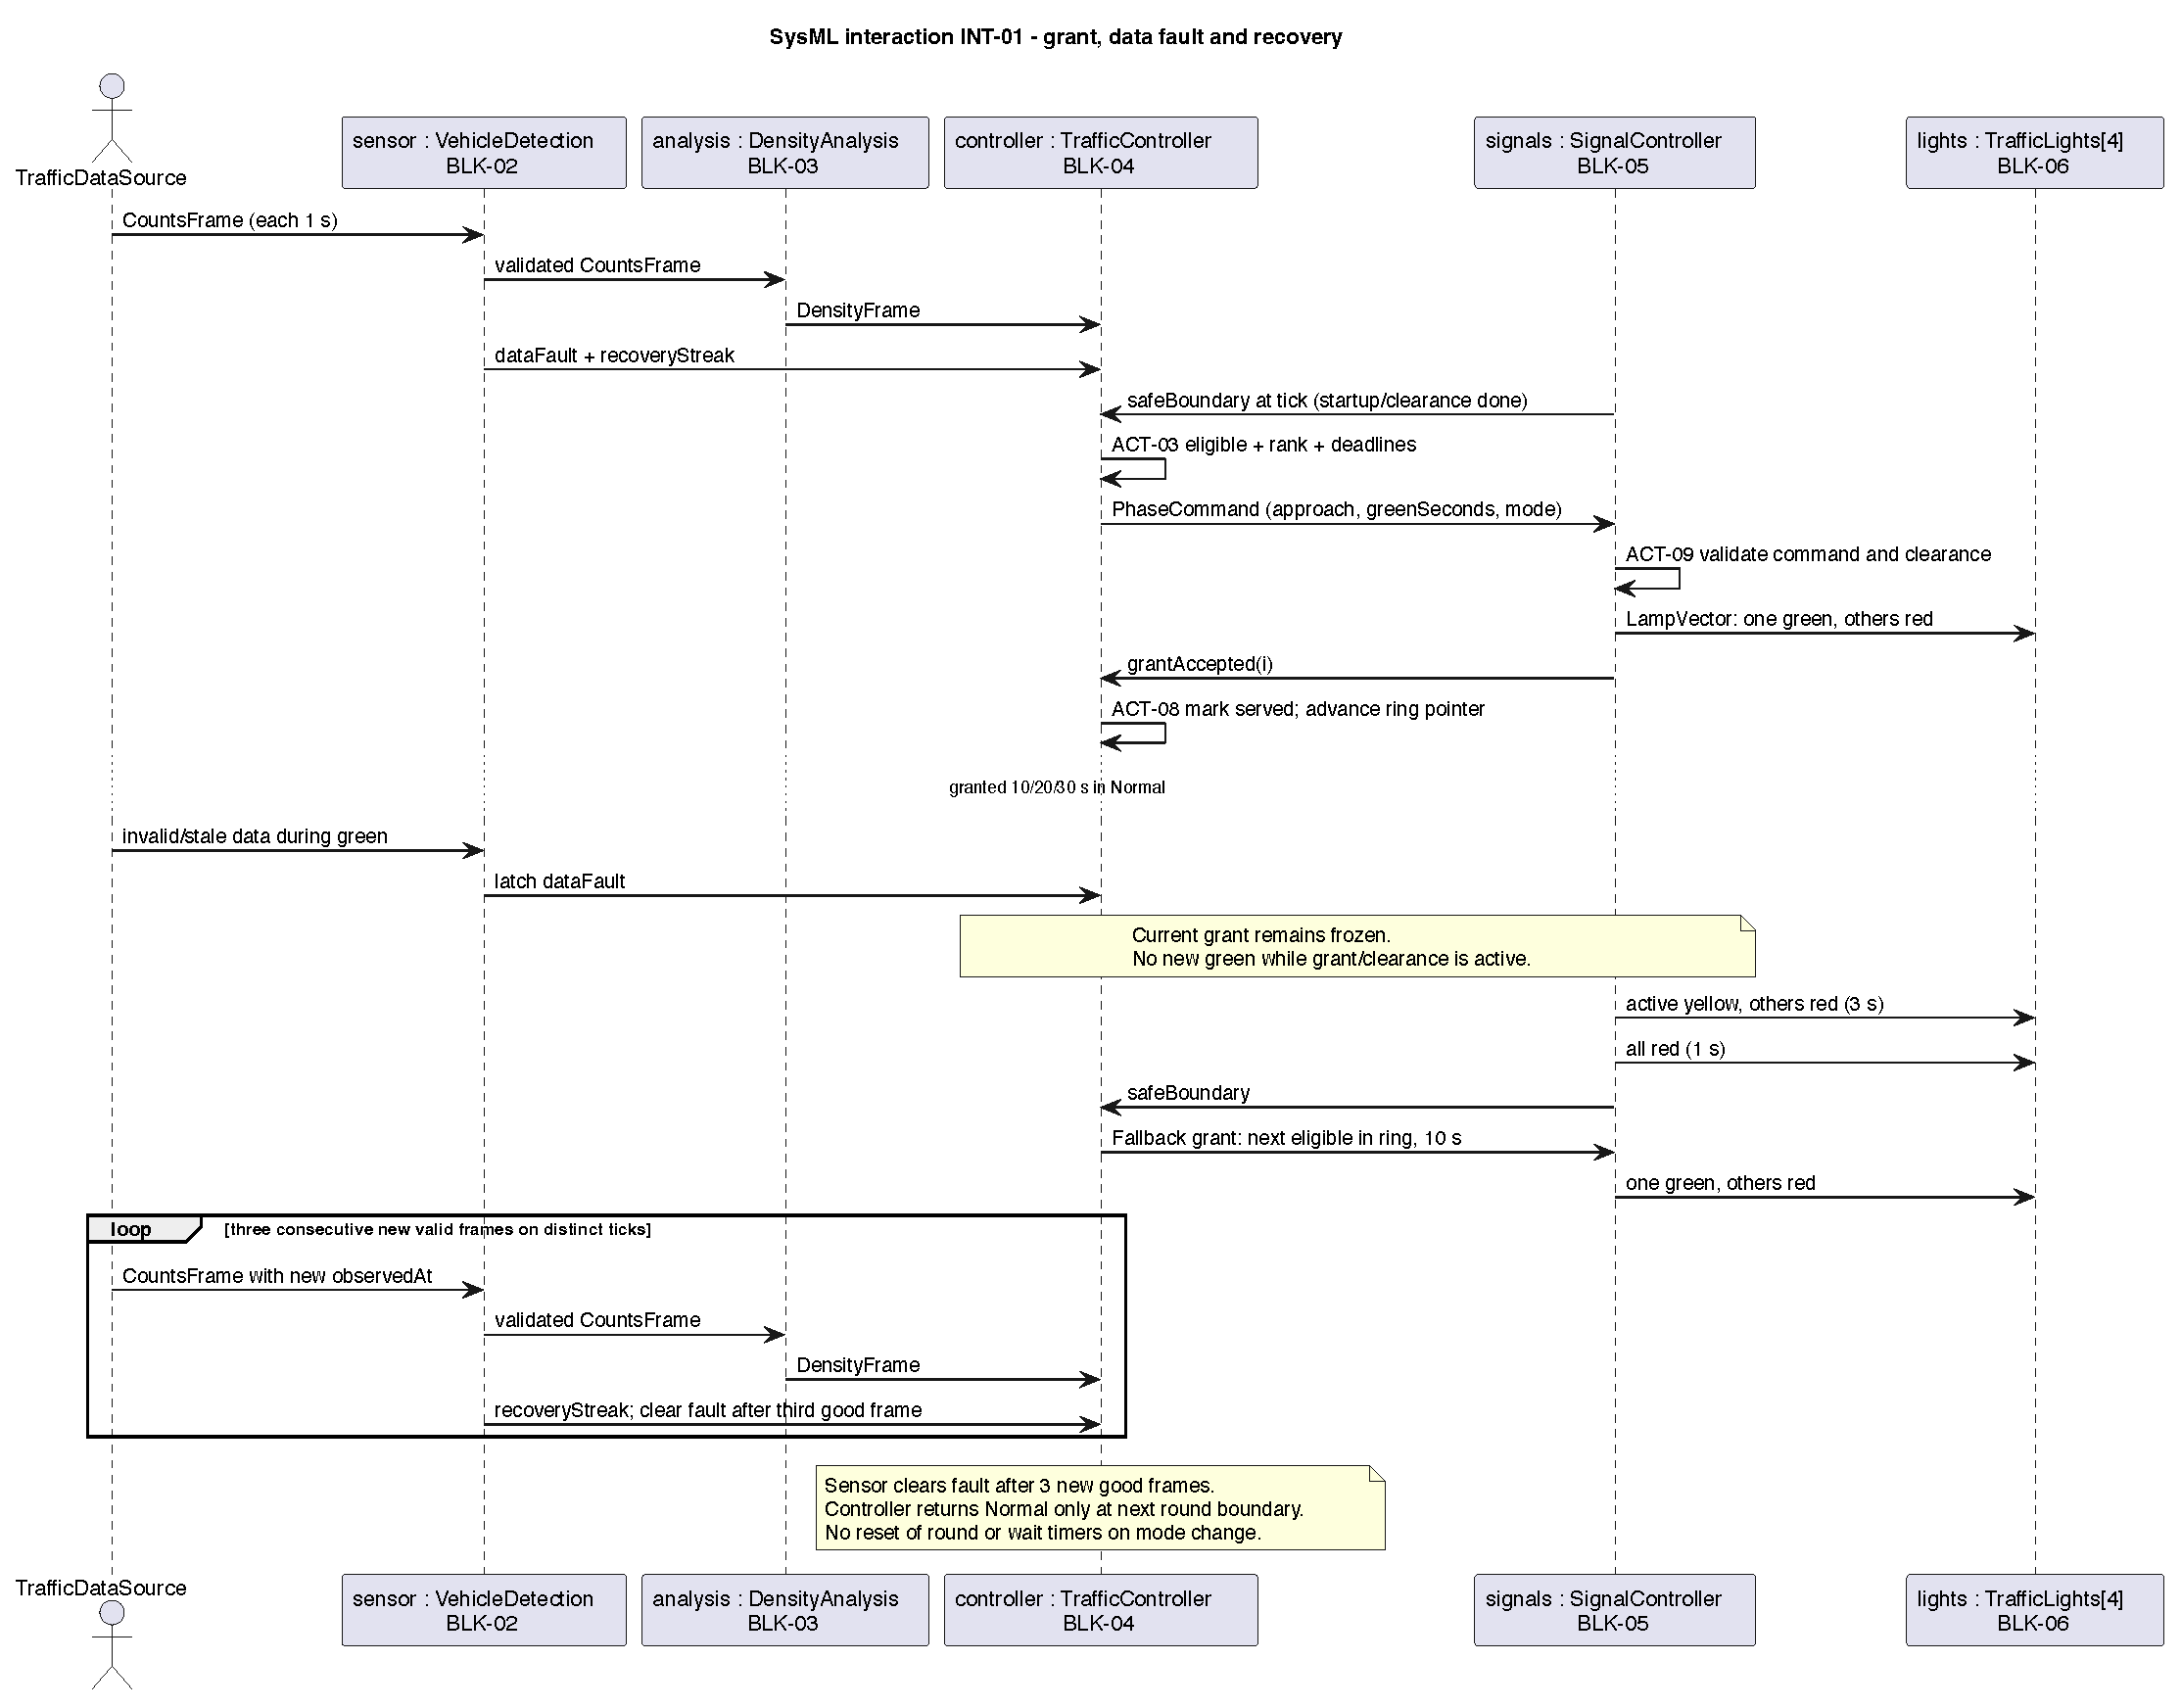
\includegraphics[width=\linewidth,height=.66\textwidth,keepaspectratio]{sequence.pdf}
\caption{Sequence view dari model baseline}\label{fig:sequence}
\sumber{Pemodelan proyek berdasarkan asumsi desain ASM-001--010 (2026)}
\end{figure}
\clearpage
\end{landscape}
\clearpage
\section{State machine view}
STM-01 dimiliki SignalController. Normal/Fallback merupakan variabel controller, bukan region sinyal concurrent. SafetyHold berada di luar composite Running dan keluar hanya melalui restart.
\begin{figure}[htbp]\centering
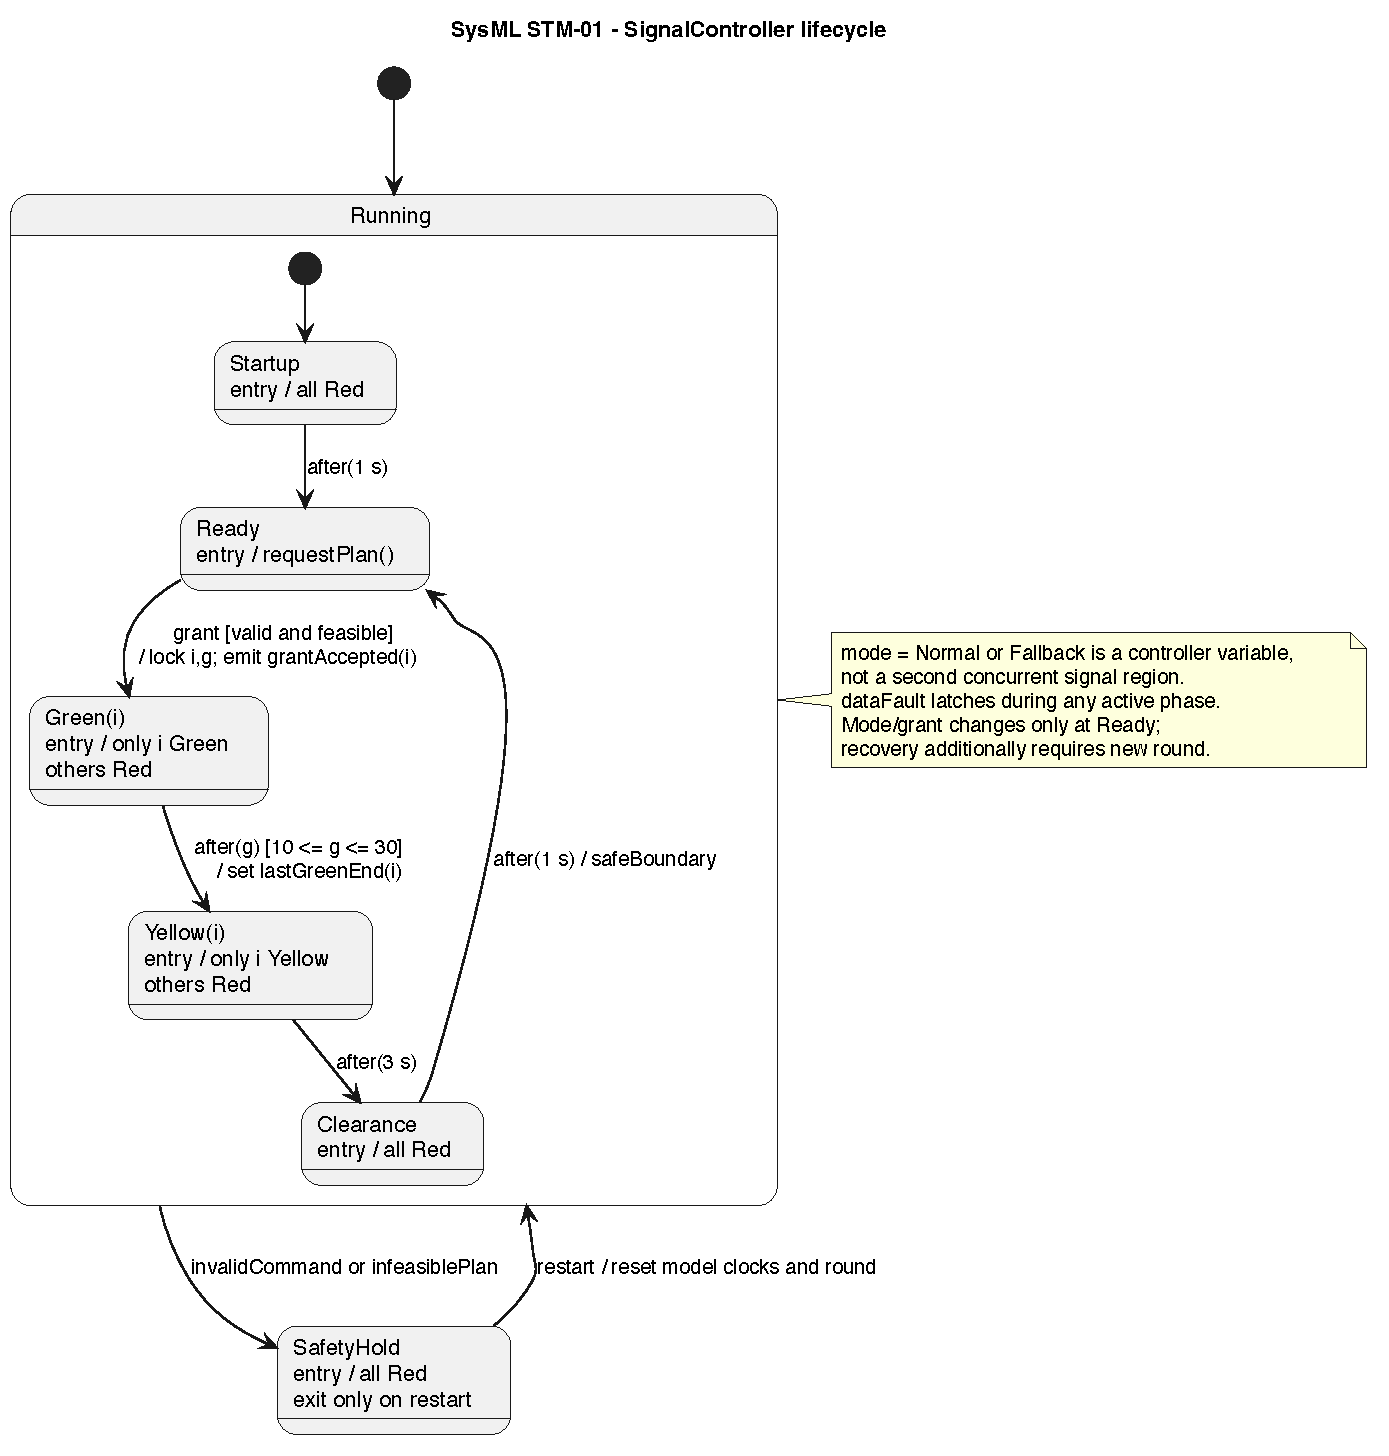
\includegraphics[width=\linewidth,height=.76\textheight,keepaspectratio]{state-machine.pdf}
\caption{State machine view dari model baseline}\label{fig:state-machine}
\sumber{Pemodelan proyek berdasarkan asumsi desain ASM-001--010 (2026)}
\end{figure}
\clearpage
\clearpage
\begin{landscape}
\section{Block Definition Diagram}
BDD mendefinisikan tipe BLK-01 sampai BLK-06 dan composition part dengan multiplicity. InterfaceBlock/value types didefinisikan dalam dictionary model; port receiver memakai conjugation.
\begin{figure}[htbp]\centering
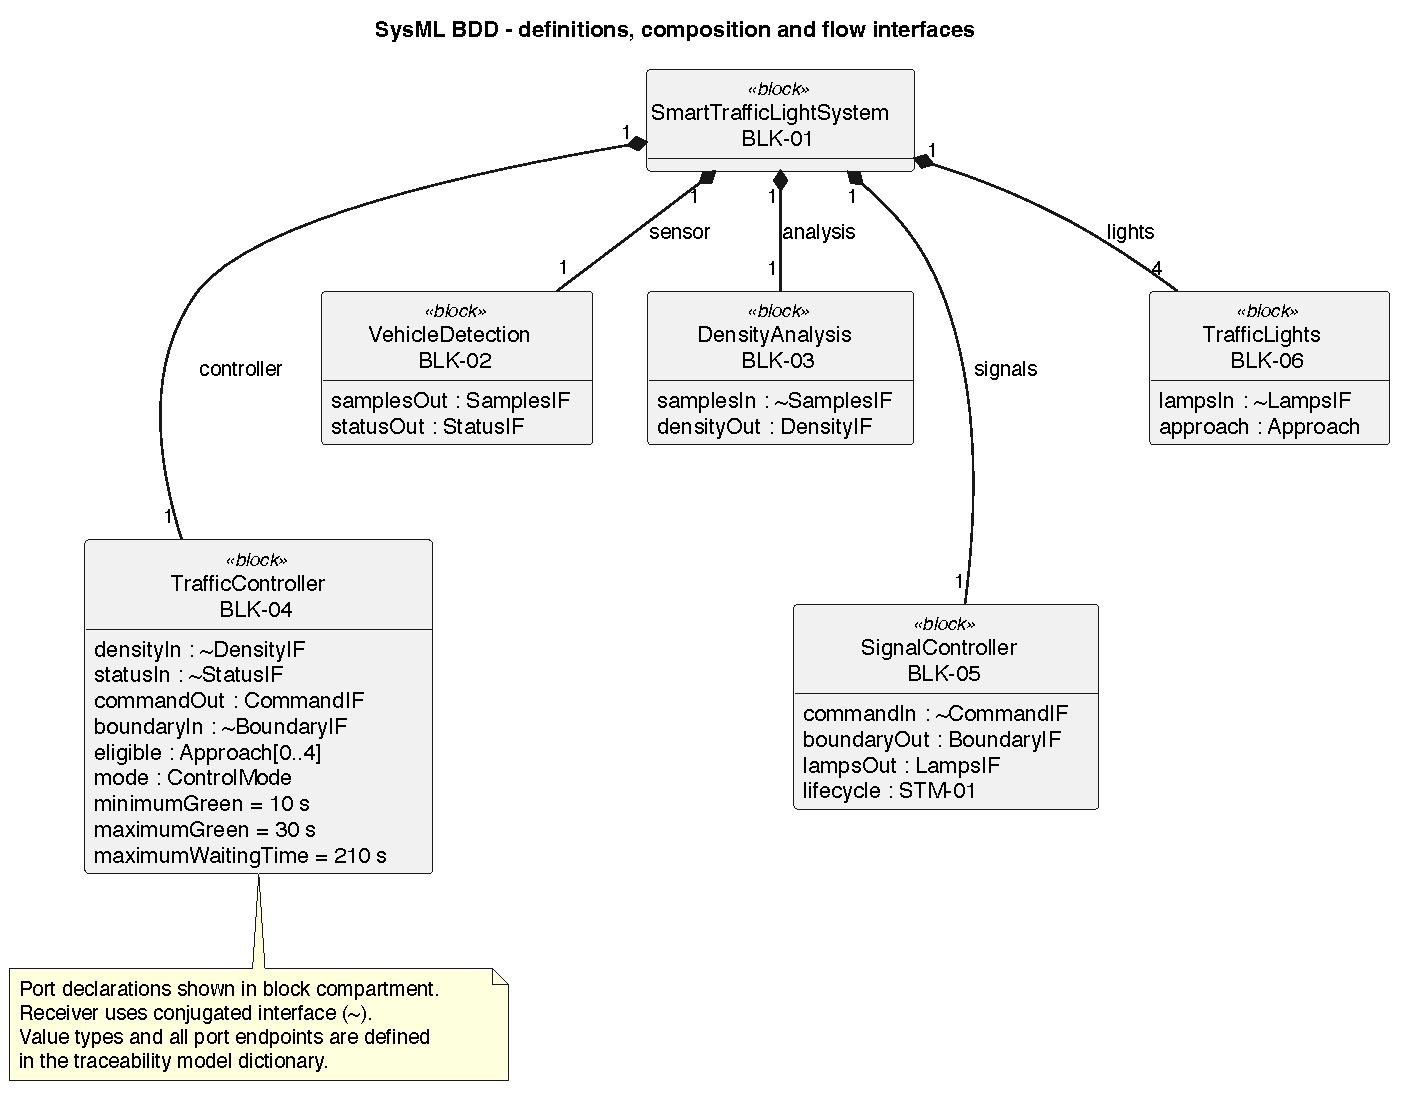
\includegraphics[width=\linewidth,height=.66\textwidth,keepaspectratio]{bdd.pdf}
\caption{Block Definition Diagram dari model baseline}\label{fig:bdd}
\sumber{Pemodelan proyek berdasarkan asumsi desain ASM-001--010 (2026)}
\end{figure}
\clearpage
\end{landscape}
\clearpage
\begin{landscape}
\section{Internal Block Diagram}
IBD memakai part dari BDD dalam context BLK-01. P01--P12 mengacu ke port bertipe pada dictionary. C01--C06 adalah assembly connector dengan item flow; panah menunjukkan flow, bukan dependency satisfy.
\begin{figure}[htbp]\centering
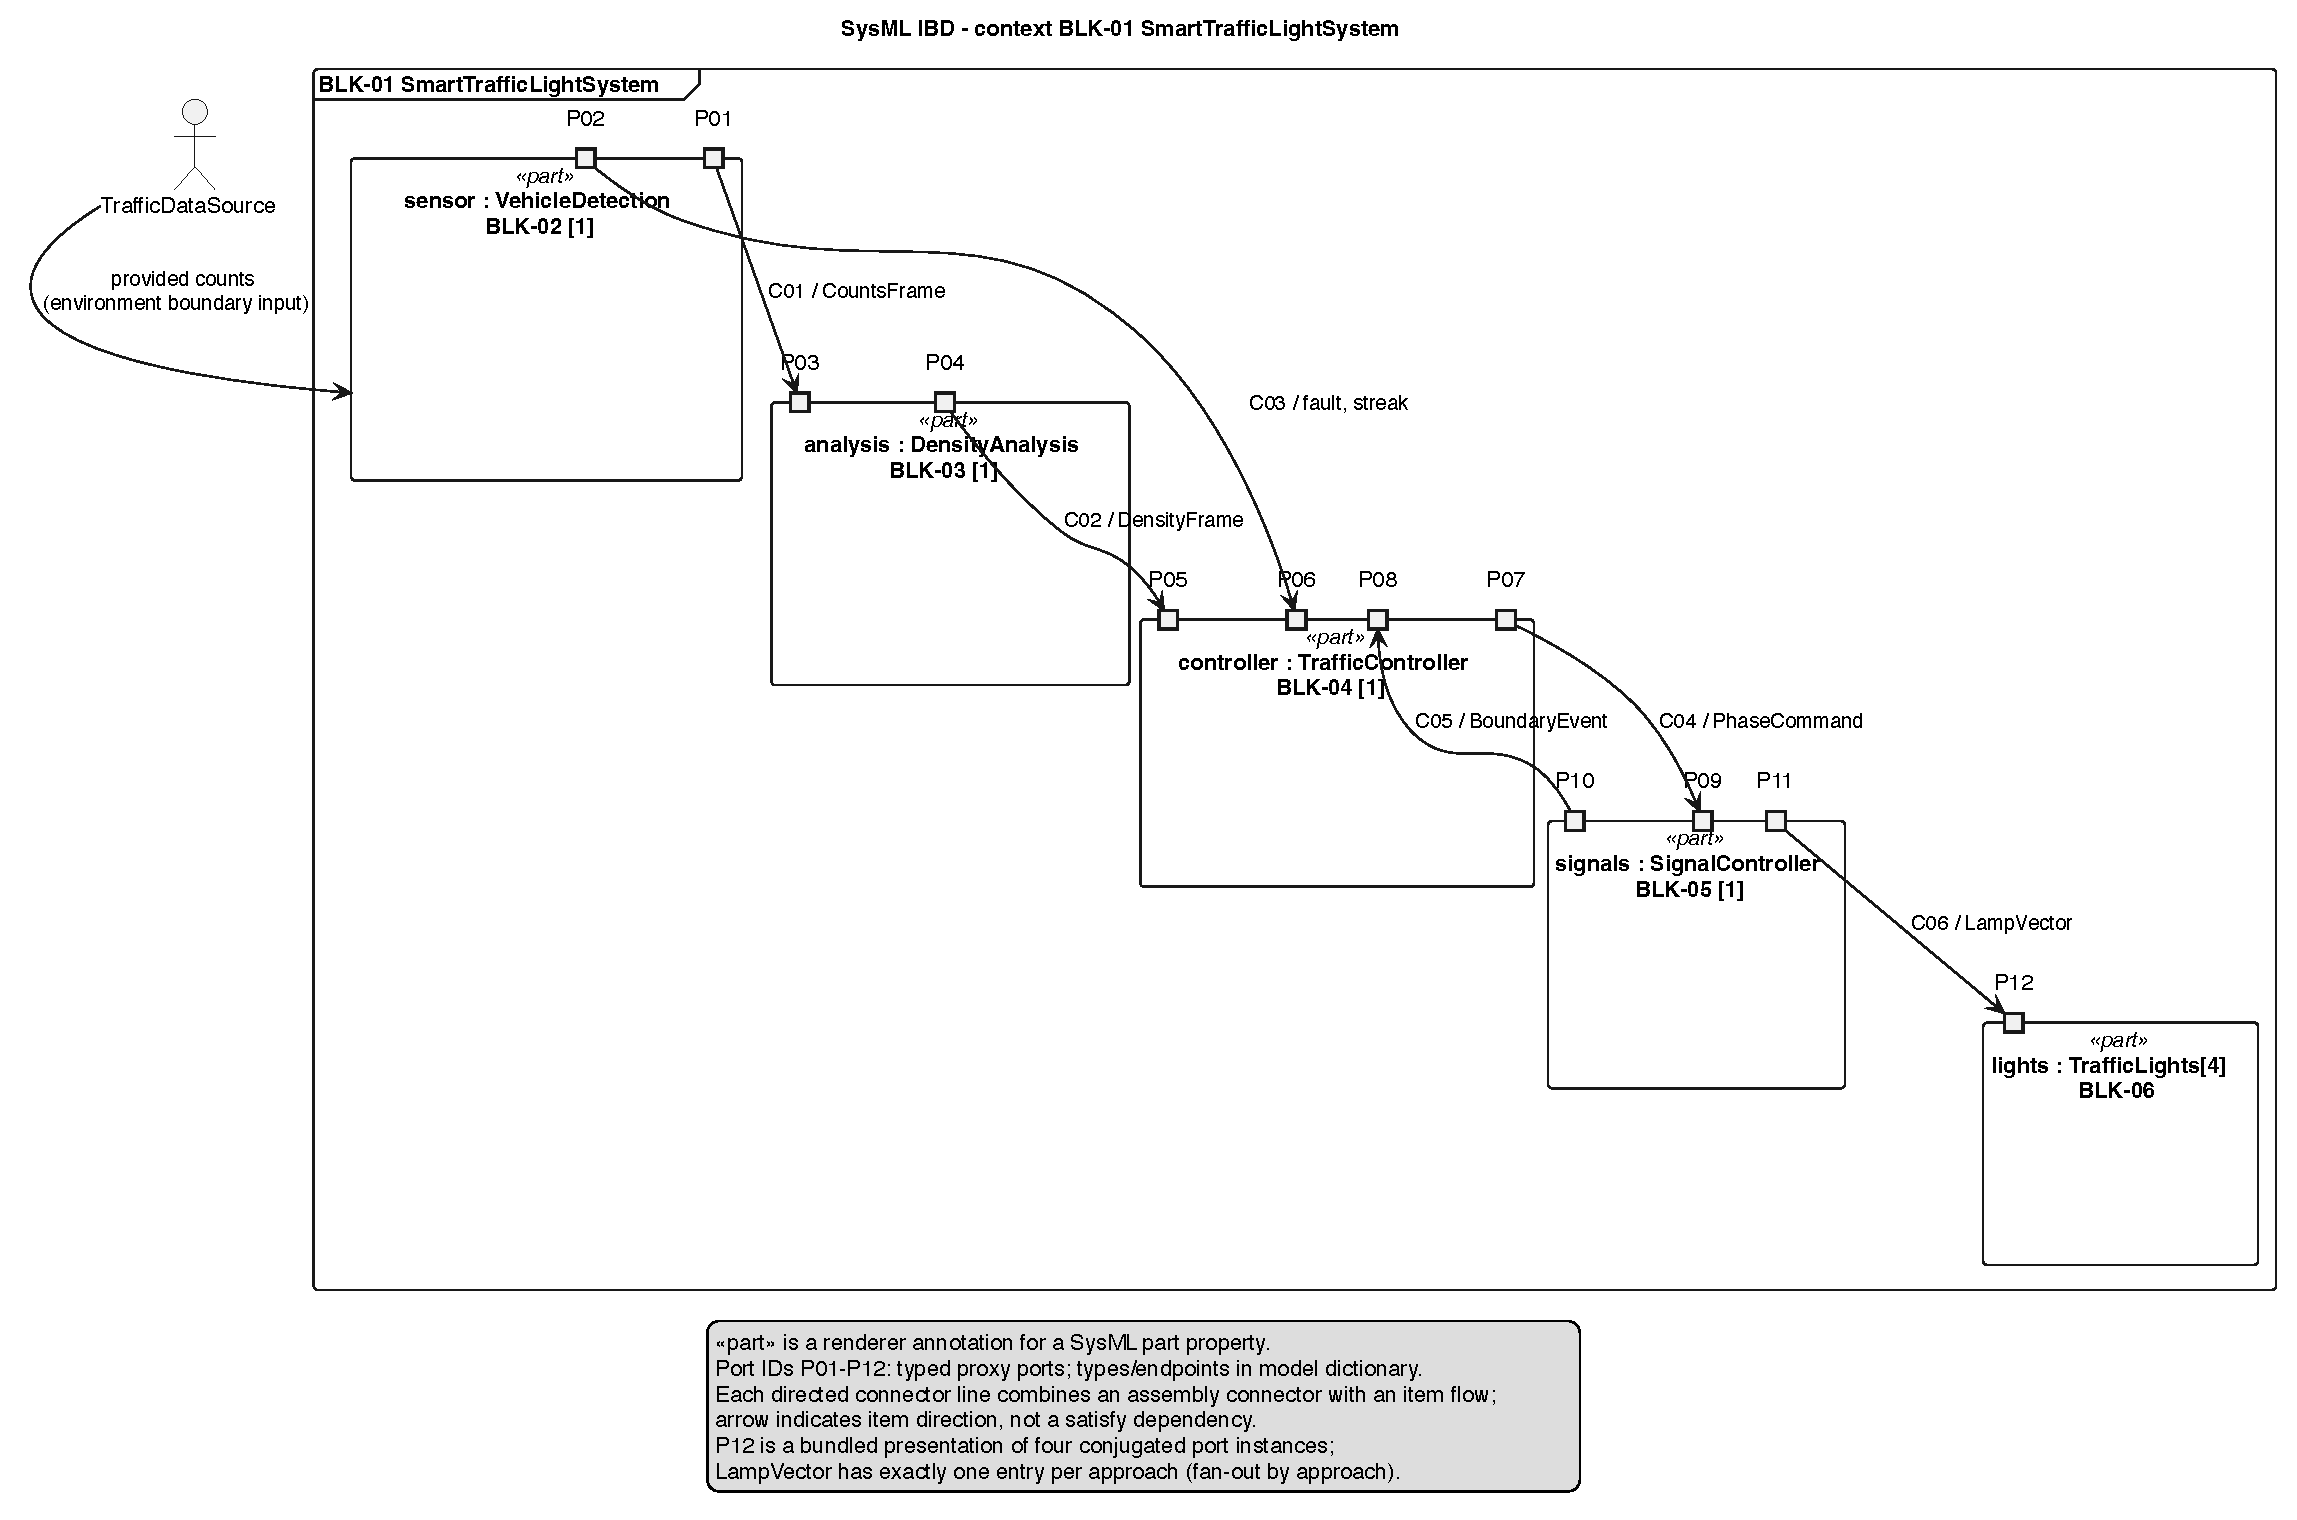
\includegraphics[width=\linewidth,height=.66\textwidth,keepaspectratio]{ibd.pdf}
\caption{Internal Block Diagram dari model baseline}\label{fig:ibd}
\sumber{Pemodelan proyek berdasarkan asumsi desain ASM-001--010 (2026)}
\end{figure}
\clearpage
\end{landscape}
